\documentclass[12pt]{article}
\usepackage[spanish]{babel}
\usepackage[utf8]{inputenc}
\usepackage{amsmath}
\usepackage{listings}
\usepackage[usenames]{color}
\definecolor{gray97}{gray}{.97}
\definecolor{gray75}{gray}{.75}
\definecolor{gray45}{gray}{.45}
\definecolor{azul1}{RGB}{141,198,163}
\definecolor{azul2}{RGB}{24,107,122}
\definecolor{verde1}{RGB}{44,186,34}
\usepackage{graphicx}
\usepackage{caption}
\usepackage{subcaption}
\usepackage{textcomp}
\lstset{
        frame=Ltb,
        framerule=1pt,
        framextopmargin=3pt,
        framexbottommargin=3pt,
        framexleftmargin=0.6cm,
        framesep=0pt,
        rulesep=.4pt,
		backgroundcolor=\color{gray97},
		rulesepcolor=,
        tabsize=4,
        rulecolor=\color[RGB]{106, 182, 217}, %AZUL
        upquote=true,
        aboveskip={1.5\baselineskip}, %despues de la linea de texto
        columns=fixed,
        showstringspaces=false,
        extendedchars=true,
        breaklines=true,
        prebreak = \raisebox{0ex}[0ex][0ex]{\ensuremath{\hookleftarrow}},
        showtabs=false,
        showspaces=false,
        showstringspaces=false,
        basicstyle=\scriptsize\ttfamily\color[RGB]{39, 100, 46}, %Numeros de lineas, simbolos, puntos y coma y demas
        identifierstyle=\ttfamily\color[RGB]{56, 140, 189}, %variables
        commentstyle=\color[RGB]{62, 179, 101}, %comentarios
        stringstyle=\color[RGB]{247, 165, 42}, %impresiones
        keywordstyle=\bfseries\color[RGB]{237, 118, 150}, %funciones
        %
		numbers=left,
		numbersep=5pt,
		numberstyle=\tiny,
		numberfirstline = false,
		breaklines=true,
		}
\usepackage{graphicx}
\usepackage[colorinlistoftodos]{todonotes}
\usepackage{natbib} %citas bibliograficas estilo APA :p
\usepackage{eso-pic}
\usepackage{avant}
\usepackage[top=2cm,bottom=2cm,left=2.5cm,right=3cm,headsep=8pt,a4paper]{geometry}
\usepackage{fancyhdr}
\pagestyle{fancy}
\fancyhf{}
%\fancyhead[LE,RO]{}
\fancyhead[RE,LO]{Procesamiento de Señales II}
\fancyfoot[CE,CO]{\leftmark}
\fancyfoot[LE,RO]{\thepage}
\renewcommand{\headrulewidth}{2pt}
\renewcommand{\footrulewidth}{1pt}
\usepackage{hyperref}
\usepackage{tabu}
\usepackage{array}
\usepackage{multirow}
\usepackage{amssymb}
\usepackage{makeidx}
\graphicspath{ {images/} }
\usepackage{wrapfig}
\usepackage{enumerate}
\usepackage{amsmath,tikz}
\usetikzlibrary{matrix}
\usepackage{steinmetz}
\newcommand*{\horzbar}{\rule[0.05ex]{2.5ex}{0.5pt}}
\usepackage{calc}
\date{\today}


\begin{document}

\begin{titlepage}
\newcommand{\HRule}{\rule{\linewidth}{0.5mm}} 
\center
\textsc{\LARGE  Benemérita Universidad \\[0.2cm] Autónoma de Puebla}\\[1.5cm] 

\includegraphics[width=4cm]{escudo.jpg}\\[1cm]
\textsc{\Large Facultad de Ciencias de la Electrónica}\\[0.5cm] 
\textsc{\large Licenciatura en Electrónica}\\[0.5cm]
\HRule \\[0.4cm]
{ \huge \bfseries Proyecto Final: FFT}\\[0.4cm] 
\HRule \\[1.5cm]
\begin{minipage}{\textwidth}
\center 

\emph{Profesor:} \\
Fernando López Marcos \\[1cm]

\begin{tabular}{ll}
\emph{Alumnos:} & \emph{Número de Matrícula:}\\
Hanan Ronaldo Quispe Condori  & 555010653 \\
Erick Sandro Niño García & 201631150\\
Carlos Alfredo Vega Aguilar & 201632131 \\
\end{tabular}
\end{minipage}\\[2cm]
\today
\end{titlepage}

%\newpage
%~\vfill
%\thispagestyle{empty}
%\begin{figure}[hbtp]


%\includegraphics[width=4cm]{IMAGENES/motordc}
%\end{figure}
%\noindent \textsc{Trabajo Encargado: Problemas en MatLab \\ Máquinas Eléctricas \\ Universidad Nacional de San Antonio abad del Cusco}\\
%noindent \textsc{Ingeniería Electrónica }\\
%\noindent \textit{Tercera revisión, \today}

%\tableofcontents indice bloqueado xD

\newpage

\section{Introducción}
El análisis espectral de una señal digital tiene por objeto la descomposición de dicha señal en sus diversas componentes dentro del dominio frecuencial. Este análisis, que puede llevarse a efecto en un ordenador (vía software) o en un sistema digital con un hardware específico, es una técnica ampliamente utilizada en varias especialidades de ingeniería, ciencias aplicadas, y procesamiento de datos. Una tarea muy común en el análisis espectral es tratar de encontrar una determinada señal que está contaminada por otras, por ejemplo ruido.
\\
\\
La FFT, a causa de su rapidez, es la herramienta más adecuada para llevar a cabo un análisis espectral. Cualquier algoritmo para calcular la FFT contiene un conjunto de coeficientes espectrales, armónicos, que se pueden entender como muestras de la correspondiente función espectral continua (Transformada continua de Fourier ).
\\
\\
Toda señal periódica puede ser representada por la suma de series de Fourier. Con un análisis adecuado es posible obtener una representación de Fourier para señales de duración finita. Esta representación es la que se conoce como la Transformada de Fourier Discreta (TFD). La TFD se puede representar como: 
\begin{equation}
    X[k] = \sum_{n=0}^{N-1} x[n] \cdot W_N^{kn}  .................     k=0,1,..., N-1
\end{equation}

Se puede observar que su resolución directa implica N multiplicaciones complejas y N-1 adiciones complejas por cada k. Para valores pequeños de N la resolución en sí no consume mucho tiempo ni recursos. Sin embargo, para valores de N lo suficientemente grandes el cálculo directo se torna poco eficiente, no solo por el gran tiempo que consume sino también por el acaparamiento de los recursos necesarios. Por ejemplo, para $N = 2^{30}$ las operaciones a realizar serían $2^{60}$; asumiendo que cada operación toma aproximadamente 1 ns, el cálculo de la TFD tardaría unos 13343 días. 
\\
\\
Tomando en cuenta esta importante desventaja, aparece la Transformada Rápida de Fourier (FFT por sus siglas en inglés), un algoritmo para el cálculo eficiente de la TFD. Su importancia radica en el hecho de que elimina una gran parte de los cálculos repetitivos a los que se ve sometida la TFD. El algoritmo de la FFT fue originalmente inventado por Carl Friedrich Gauss en 1805. Diferentes versiones del algoritmo fueron descubiertas a lo largo de los años, pero la FFT no se hizo popular sino hasta 1965, con la publicación de James Cooley y John Turkey, quienes reinventaron el algoritmo al describir como ejecutarlo de forma eficiente en una computadora.
\section{Objetivos}
Que el alumno implemente y optimice el algoritmo de la Transformada Discreta de Fourier y lo compare con los algoritmos interconstruidos de la Transformada Rápida de Fourier. 
\\
\\

\section{Desarrollo}
La idea básica detrás de la FFT consiste en la división del tiempo, es decir, en la descomposición iterativa en Transformadas de Fourier Disscretas más simples. La FFT hace uso de dos propiedades de la TFD. La FFT asume que N es potencia de 2, sin embargo, existen métodos para adaptar otros valores de N a las condiciones necesarias de este algoritmo. 
\\
Las propiedades que se aprovechan son las siguientes:
\\
\textit{Simetría conjugada compleja:}
$$W_{N}^{k(N-n)} = W_{N}^{-kn} = (W_{N}^{k+N}) ^{*}$$
\textit{Periodicidad en n,k:}
$$W_{N}^{kn} = W_{N}^{k(N +n)} = W_{N}^{(k+N)n}$$
La FFT divide la Transformada de Fourier Discreta a calcular en dos TFD menores según la paridad de los términos:
$$X[k] = \sum_{n=0}^{N-1} x[n] \cdot W_{N}^{kN} = \sum_{r=0}^{(N/2)-1} x[2r] \cdot W_{N}^{2rk} + \sum_{r=0}^{(N/2)-1} x[2r+1] \cdot W_{N}^{(2r+1)k} ..... r=0,1,..., \dfrac{N}{2} -1$$
$$X[k] = \sum_{r=0}^{(N/2)-1} x[2r] \cdot (W_{N}^{(2)})^{rk} + W_{N}^{K} \sum_{r=0}^{(N/2)-1} x[2r+1] \cdot (W_{N/2})^{rk}$$
Sabiendo que $W_{N}^{2} = e^{-j\dfrac{2\pi}{N/2}} = W_{N/2}$ se puede re-expresar la TFD de N muestras en la suma de dos TFD de N/2 muestras[\cite{deergha2018digital}].
\begin{equation}
    X[k] = \sum_{r=0}^{(N/2)-1} x[2r] \cdot (W_{N/2})^{rk} + W_{N}^{K} \sum_{r=0}^{(N/2)-1} x[2r+1] \cdot (W_{N/2})^{rk}
\end{equation}

Dado que se tratan de dos TFD, esto significa que podemos aplicar el mismo método de división en pares e impares para así obtener dos pares de TFD de N/4 muestras. El método es así aplicado hasta que se obtienen TFD de 1 muestra, cuyo cálculo resulta sencillo. Una vez obtenidos los valores de las TFD simples, es cuestión de adicionar los resultados. 
\\
Se puede observar que si se tenía inicialmente una TFD de N muestras, se podrán llevar a cabo $p = log_{2} N$ divisiones. Si calculamos el costo de las operaciones que hay que llevar a cabo con este método, se tiene que el algoritmo es de complejidad ($N \cdot log_{2} N$).\\\\
\subsection{Implementación de la TFD y FFT}
Para implementar la TFD se usa explicitamente la fórmula (1). En el siguiente código se muestra su implementación
\lstinputlisting[language=Matlab]{midft.m}
Para implementar la FFT se recurrió a la propiedad (3) que es un caso especial de la propiedad (2).
\begin{equation}
    X[k]=X^{*}[N-K]
\end{equation}
El código se muestra a continuación
\lstinputlisting[language=Matlab]{mifft.m}
La propiedad (3) aprovecha la simetría que se muestra en la figura \ref{fig:comparacion}.

\begin{figure}[h!]
 \centering
 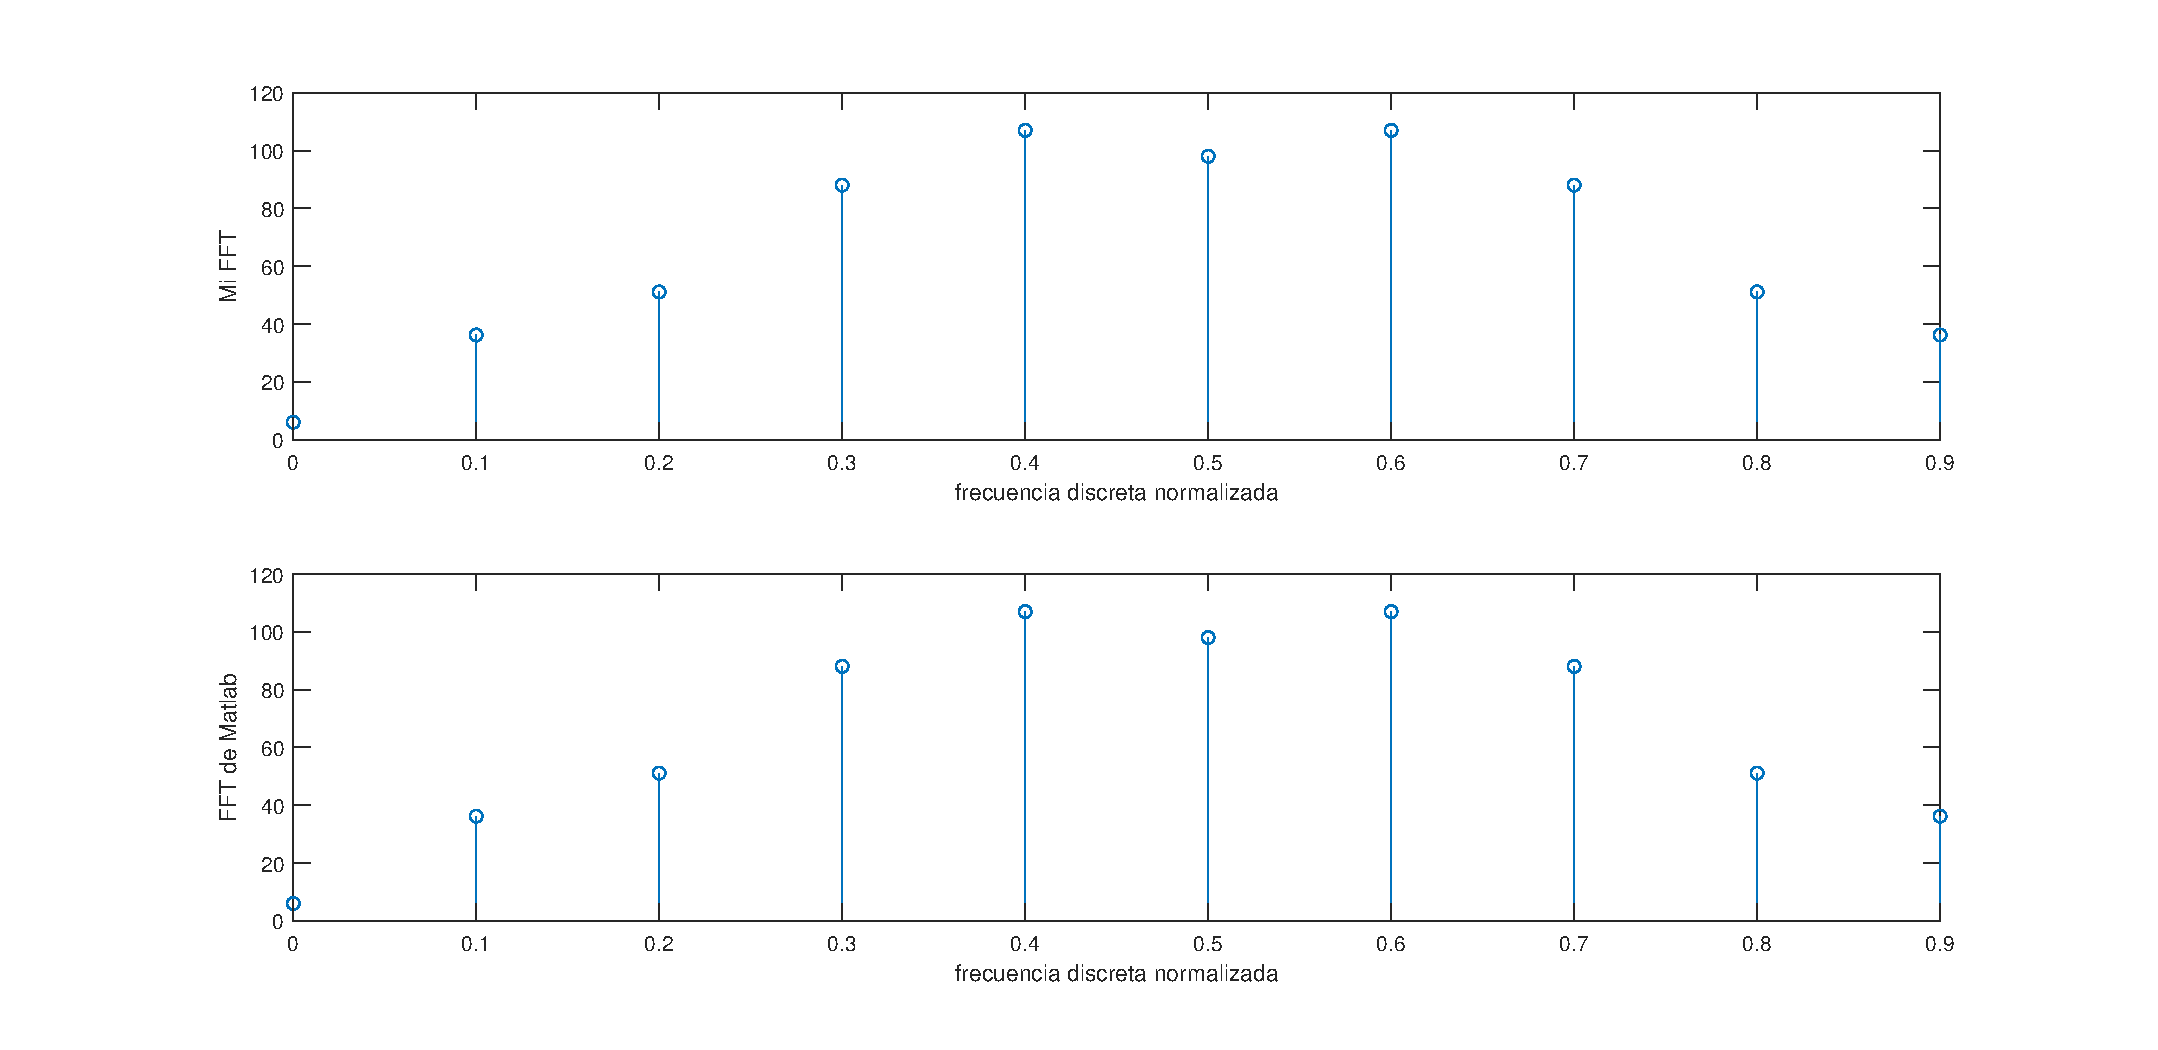
\includegraphics[width=1\textwidth]{ima1.eps}
 \caption{TFD implementada vs FFT de MATLAB en frecuencia normalizada}
 \label{fig:comparacion}
\end{figure}

Donde se observa que existe un eje de simetría en la frecuencia central $0.5$. Así solo se debe de calcular la mitad de los valores de la TFD. Es importante descartar le coeficiente en la frecuencia $0$  para conservar la simetría ya que representa la componente en CD.
\subsection{Procedimiento para corroborar la TFD Y FFT implementadas}
\subsubsection{TFD de 100 puntos}
Se implementó la TFD y FFT  de 100 puntos en dos señales: una señal sinusoidal y una señal cuadrada. En la figura 2 se muestra la señal sinusoidal a $441$ Hz de frecuencia con una frecuencia de muestreo de $44100$ Hz.
\begin{figure}[h!]
 \centering
 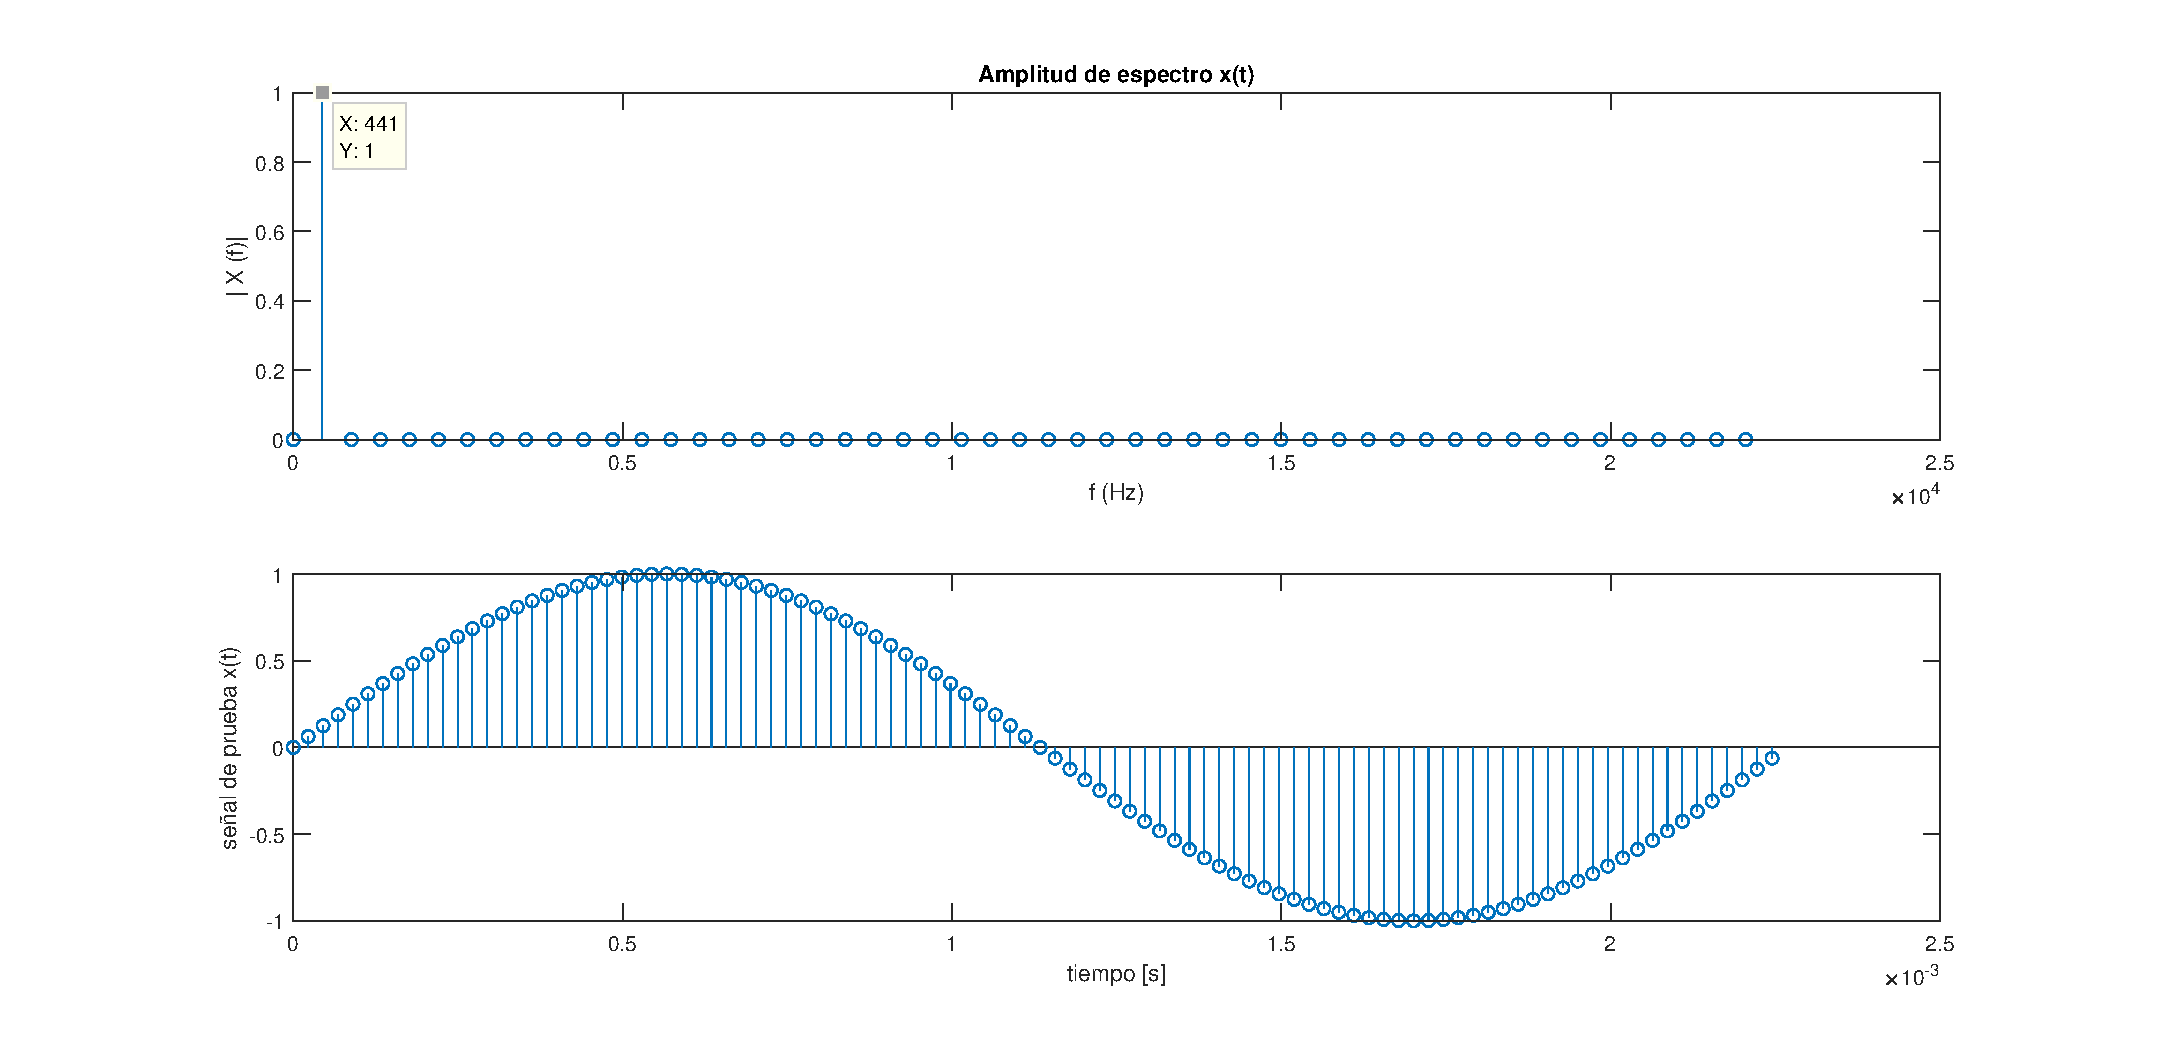
\includegraphics[width=1\textwidth]{ima2.eps}
 \caption{TFD de una señal sinusoidal}
 \label{fig:comparacion}
\end{figure}
En la figura 3 se muestra la señal cuadrada con un duty cicle del $50\%$ con una frecuencia de $4410$ Hz y una frecuencia de muestreo de $44100$ Hz.
\begin{figure}[h!]
 \centering
 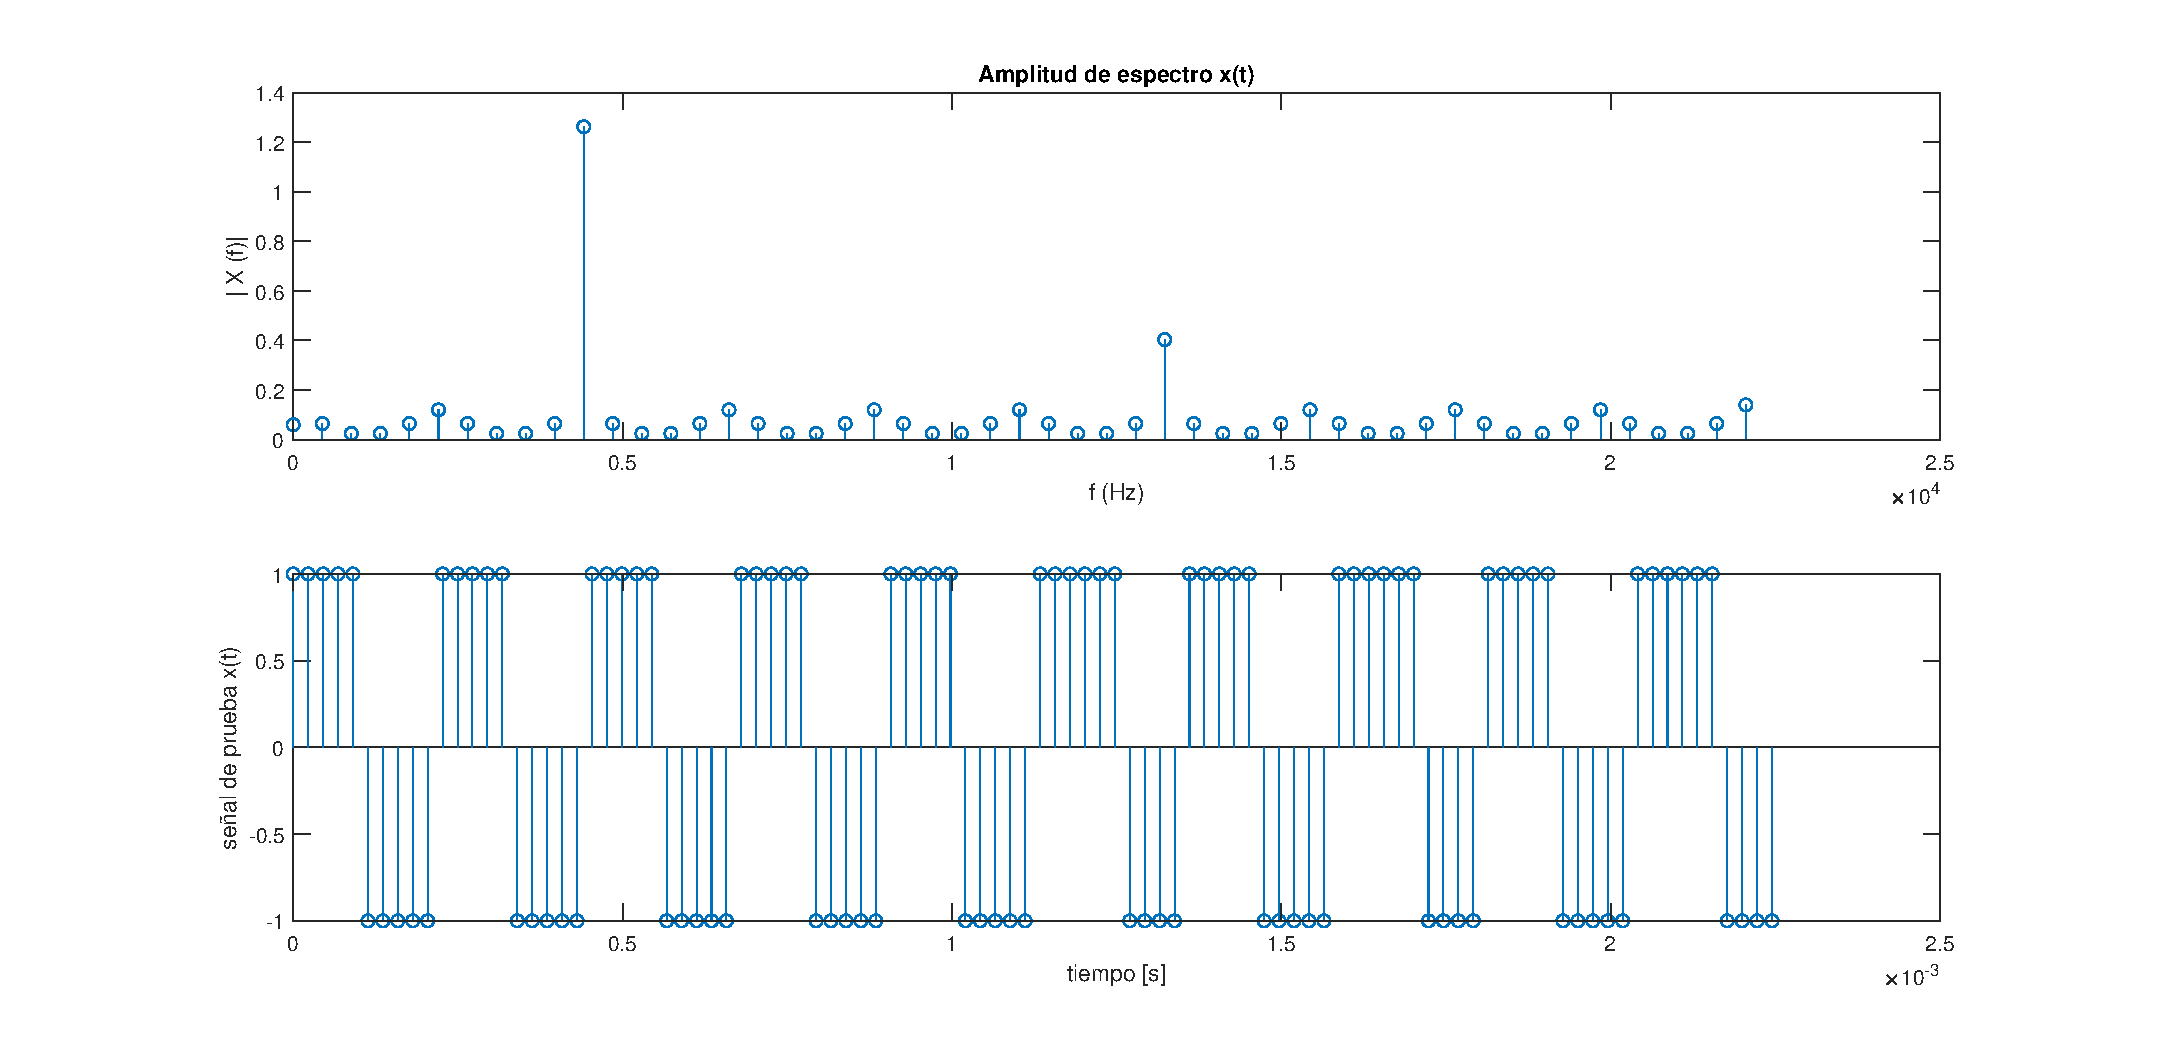
\includegraphics[width=1\textwidth]{ima3.eps}
 \caption{TFD de una señal cuadrada}
 \label{fig:comparacion}
\end{figure}
En la figura 4  se muestra el tiempo de ejecución de la TFD y la FFT diseñadas en comparación con la FFT de MATLAB.
\begin{figure}[h!]
 \centering
 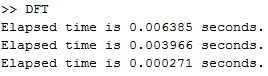
\includegraphics[width=.3\textwidth]{seno.PNG}
 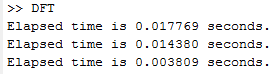
\includegraphics[width=.3\textwidth]{cuadrada.PNG}
 \caption{IZQUIERDA: En la parte superior se tiene el tiempo de ejecución de la TFD  implementada, en medio se tiene el tiempo de la FFT implementada y abajo se tiene el tiempo de la FFT de Matlab para la señal senoidal. DERECHA: Se tiene el mismo orden que en la imagen de ARRIBA pero en este caso se trada de la señal cuadrada}
 \label{fig:comparacion}
\end{figure}
\subsubsection{TFD de 128 puntos}
Se implemento nuevamente la TFD y la FFT diseñadas junto con la FFT de MATLAB pero con 128 puntos. Se tomó 100 valores de la señal y 28 valores constantes para crear un vector de 128 valores. Las constantes se determinaron con el valor de $0$. En la figura 5 se muestran las señales sinusoidal y cuadrada con sus respectivas transformadas discretas de fourier.
\begin{figure}[h!]
 \centering
 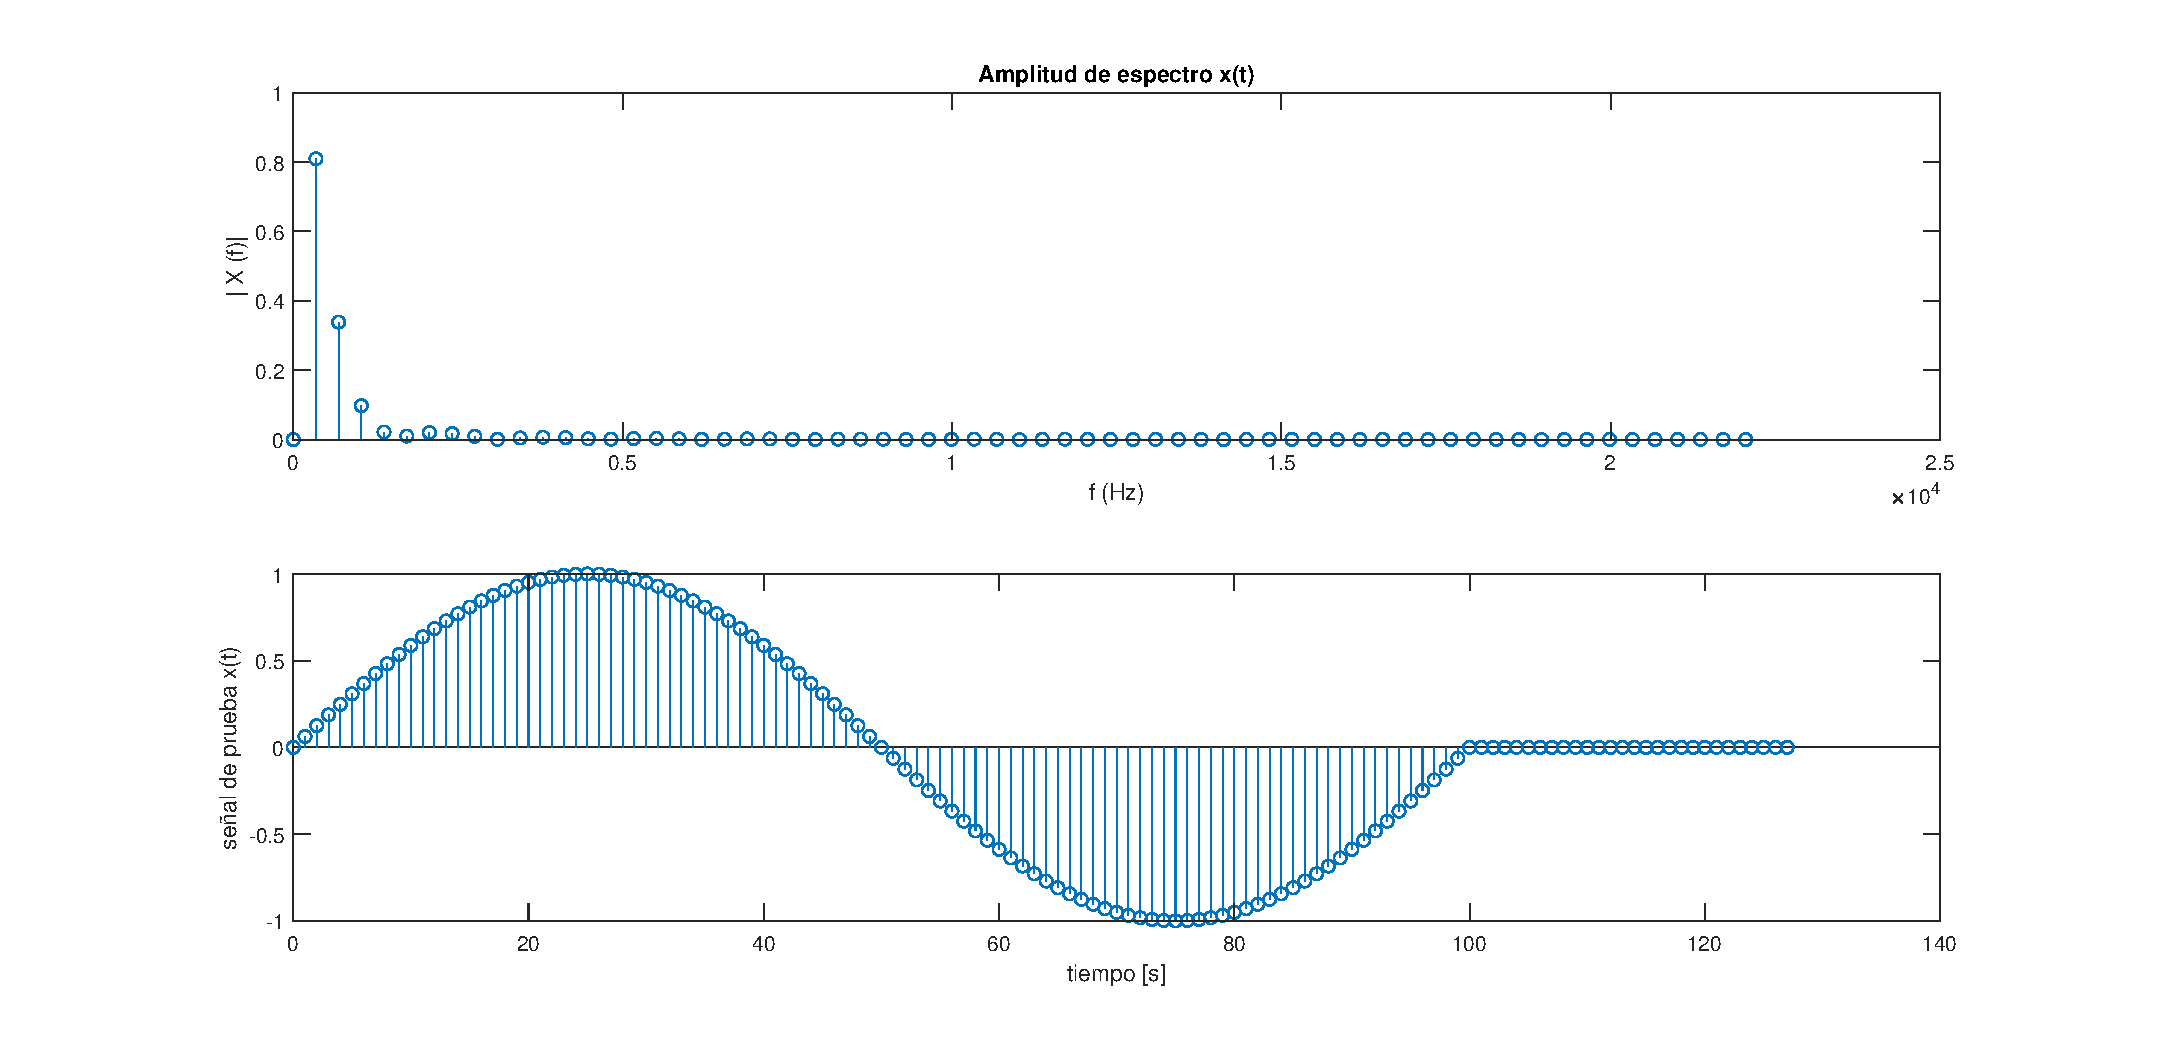
\includegraphics[width=1\textwidth]{ima4.eps}
 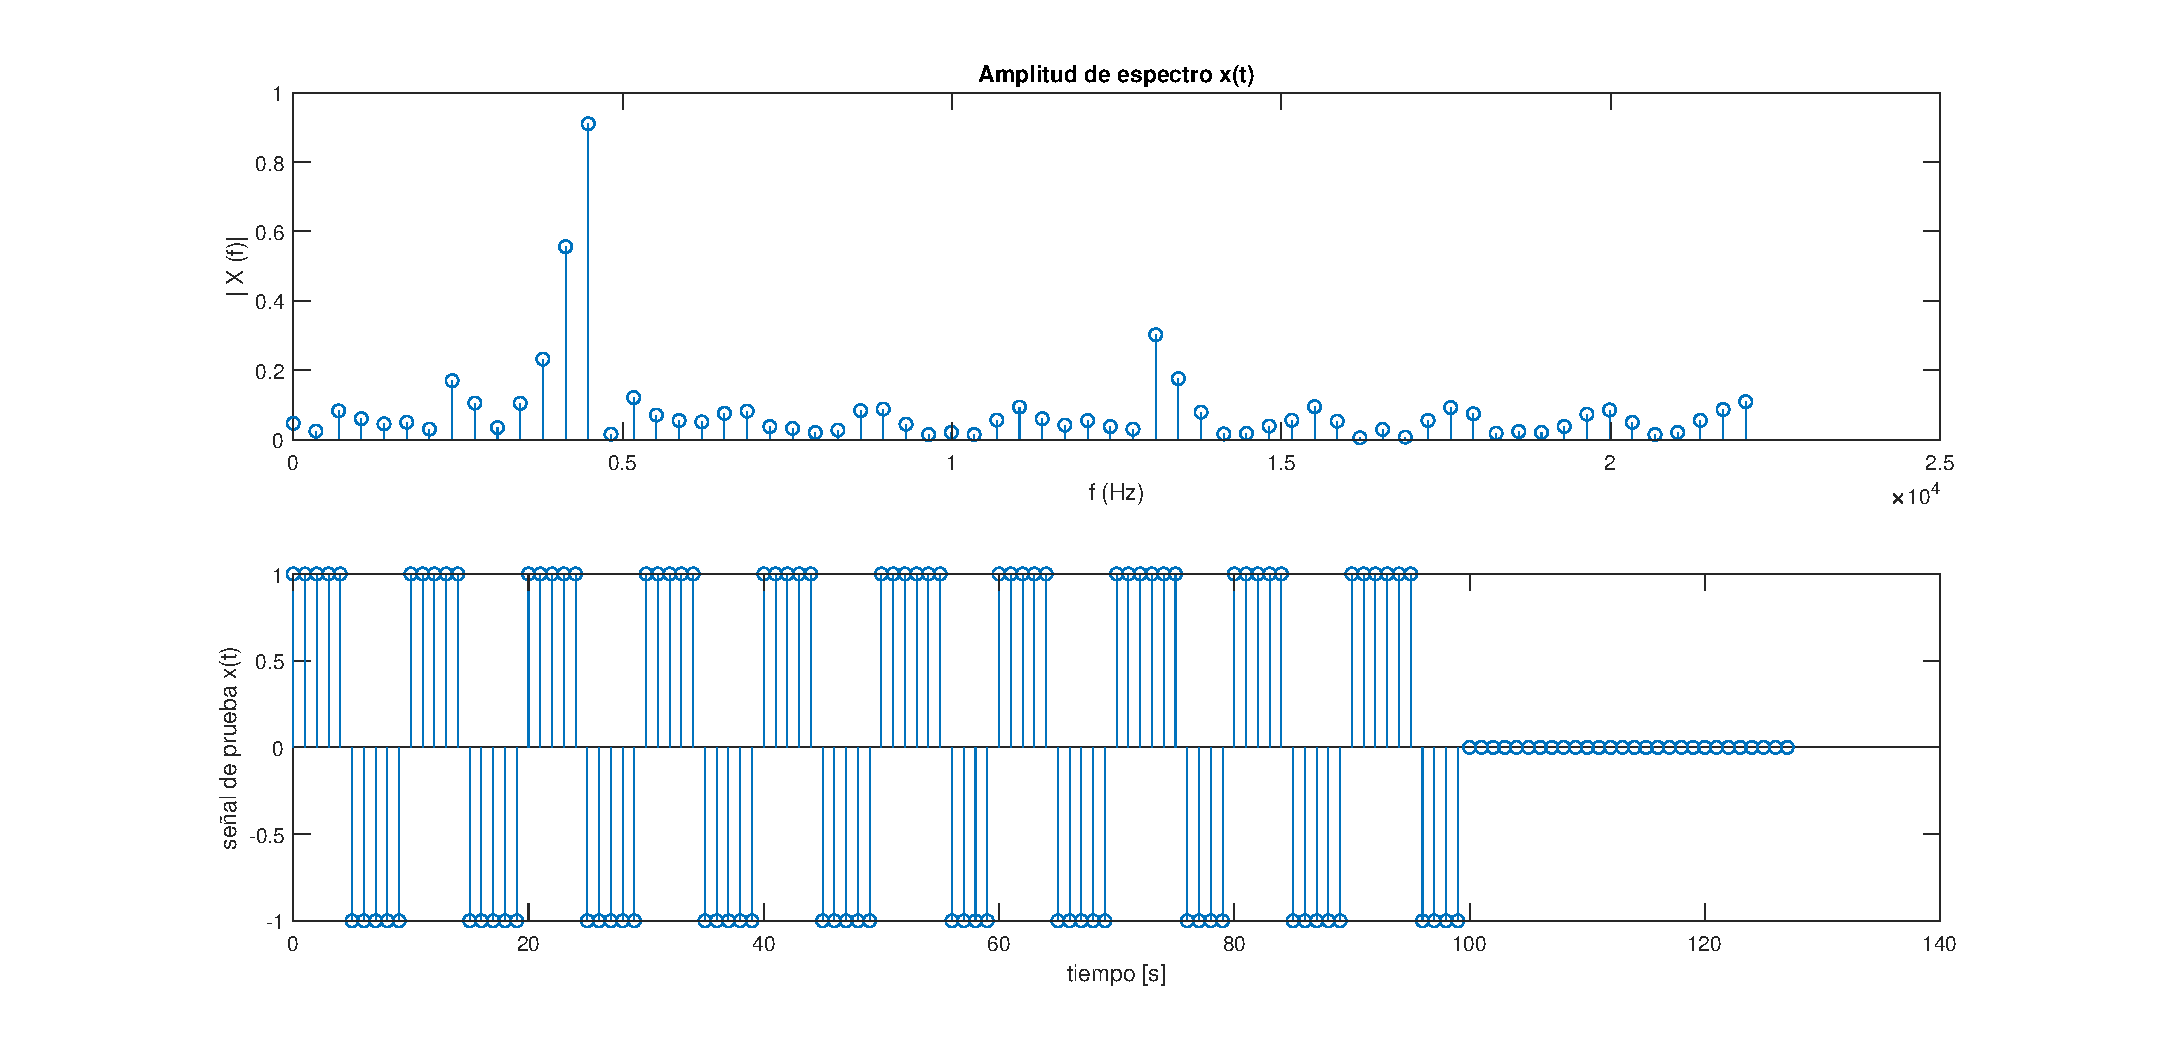
\includegraphics[width=1\textwidth]{ima5.eps}
 \caption{ARRIBA: señal sinusoidal y su TDF. ABAJO: señal cuadrada y su TDF.}
 \label{fig:comparacion}
\end{figure}
\newpage
El tiempo de ejecución correspondientes para las dos señales se muestran en la figura 6
\begin{figure}[h!]
 \centering
 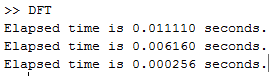
\includegraphics[width=.3\textwidth]{seno128.PNG}
 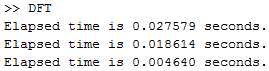
\includegraphics[width=.3\textwidth]{cuadrada128.PNG}
 \caption{IZQUIERDA: En la parte superior se tiene el tiempo de ejecución de la TFD  implementada, en medio se tiene el tiempo de la FFT implementada y abajo se tiene el tiempo de la FFT de Matlab para la señal senoidal. DERECHA: Se tiene el mismo orden que en la imagen de ARRIBA pero en este caso se trada de la señal cuadrada}
 \label{fig:comparacion}
\end{figure}
\newpage
\newpage
\section{Cuestionario}
\begin{enumerate}
    \item ¿Con qué procedimiento obtuvo el mejor resultado de tiempo y por qué?
    
    El mejor procedimiento fue la TFD optimizada ya que se realizaba la mitad de las operaciones debido a que solo se calculaban la mitad de los coeficientes de fourier. Con la propiedad (3) se determinaba la otra mitad de los coeficientes de fourier.
    
    \item¿Qué procedimiento es el más cercano a lo esperado para la señal alimentada?
    
    Ambos procedimientos ofrecen practicamente los mismos resulados como se puede observar en la figura (\ref{fig:comparacion}) por lo que se puede afirmar que ambos resultados son lo esperado para la señal de entrada. 
    
    \item¿Cuáles otros recursos de programación considera necesarios para disminuir el tiempo de ejecución de una rutina de DFT?
    
    Otras opciones de optimización se pueden encontrar en aplicar tecnicas de programación competitiva tales como \textbf{Divide and Conquer} y \textbf{Dynamic Programming}, la primera opción consiste en dividir el problema en subproblemas más simples, resolverlos y despues combinarlas en una solución general, para esto se tendria que hacer una version recursiva del algoritmo planteado, en esta versión se observaria que en cada llamada recursiva se divide el número de elementos a la mitad, el número resultante de llamadas recursivas seria por tanto $log_2N$, al combinar los resultados de estos subproblemas el tiempo de ejecución es lineal, si el tamaño de muestra es $N$ entonces el tiempo total tiene un límite de $Nlog N$ esta optimización es conocida como la FFT de Cooley–Tukey[\cite{auslander1996equivariant}].\\
    El paradigma de programación dinámica(DP) es una forma más rápida de hacer backtracking recursivo, esto se puede usar para disminuir aun más el tiempo de ejecución del algoritmo planteado[\cite{halim2013competitive}].
\end{enumerate}

\section{Conclusiones}
La Transformada Rápida de Fourier (FFT) es un algoritmo para el cálculo de la Transformada Discreta de Fourier (DFT) basado en la división del tiempo, eliminando así gran parte de los cálculos repetitivos que hay que llevar a cabo si se desea resolver la DFT de forma directa. Consideremos el ejemplo presentado inicialmente, para $N=2^{30}$ teníamos que el tiempo de cálculo total era de 13343 días. Ahora aplicando la FFT resulta que hay que realizar sólo $30*2^{30}$ operaciones; asumiendo nuevamente que cada operación tarda 1 ns tenemos que el tiempo de cálculo total es de aproximadamente 32 segundos. (Esto de manera ideal, con un algoritmo optimizado, recuerde que nuestro trabajo trata de aproximar estos tiempos con los conocimientos y recursos tecnológicos con los que el equipo cuenta).
\\
\\
Podemos concluir, que la FFT beneficia considerablemente a las aplicaciones de procesamiento de señales no sólo de forma genérica al brindar una forma más eficiente que elimina cálculos redundantes, sino también porque permite la resolución de DFT's para números grandes de muestras en situaciones en las que el método directo no es aplicable. 

\section{Apéndice}
\textbf{Código implementado para el proyecto final}
\lstinputlisting[language=Matlab]{DFT.m}
\bibliographystyle{ieeetr}
\bibliography{biblio}
\end{document}
